\documentclass[10pt,a4paper]{article}
\usepackage[utf8]{inputenc}
\usepackage[german]{babel}
%%\usepackage[babel,german=quotes]{csquotes}
\usepackage[T1]{fontenc}
\usepackage{amsmath}
\usepackage{amsfonts}
\usepackage{amssymb}
\usepackage{makeidx}
\usepackage{graphicx}
\usepackage{hyperref}
\usepackage{multirow}
\usepackage{float}
\usepackage{alltt}
\usepackage[backend=biber, %% Hilfsprogramm "biber" (statt "biblatex" oder "bibtex")
style=authoryear, %% Zitierstil (siehe Dokumentation)
natbib=true, %% Bereitstellen von natbib-kompatiblen Zitierkommandos
hyperref=true, %% hyperref-Paket verwenden, um Links zu erstellen
]{biblatex}
\usepackage{pdfpages} 

\author{Wolfgang Reder}
\title{Gleismodule}

\addbibresource{gleissymbole.bib}
\begin{document}

\maketitle
\begin{abstract}
Dieses Dokument beschreibt den physikalischen und logischen Aufbau der einzelnen Module.
\end{abstract}
\tableofcontents
\newpage
\listoffigures
\newpage
\listoftables
\newpage
\section{Hardware}
Die einzelnen Gleismodule haben eine Grundfläche von 30x30 mm und können mit bis zu 8 LED oder einem Schalter bestückt werden.

Der Schalter befindet sich immer in der mittleren Position 9. Ist der Schalter bestückt, kann an der Position 9 keine LED bestückt werden. R9 muss dann ebenfalls nicht bestückt werden.

Position 7 bleibt immer frei.
\begin{figure}[hbtp]
\centering
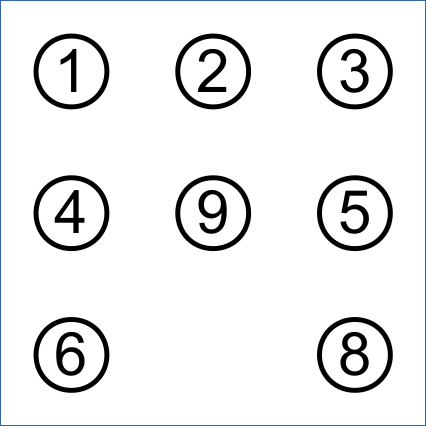
\includegraphics[width=3cm]{../folien/symbol.png}
\caption[Bestückungspositionen]{Bestückungspositionen von TOP aus gesehen}
\end{figure}

Zentrales Bauteil der Hardware ist der Microcontroller \href{https://www.microchip.com/wwwproducts/en/ATtiny804}{ATtiny804}\footcite{Microchip2019a} der Firma Microchip. Er übersetzt die Statusbefehle vom Stellwerksrechner in die entsprechende Ansteuerung der LEDs bzw. meldet eine Änderung des Tastenzustandes.

Die Kommunikation mit dem Stellwerksrechner wird über einen 5V I\textsuperscript{2}C Bus mit max. $100k\frac{bit}{s}$ Übertragungsrate hergestellt. 


\subsection{Steckerbelegung}
Die einzelnen Module werden mittels Flachbandkabel untereinander verbunden. Jede Steckerposition am Kabel ist gleich.
\begin{table}[h!]
\centering
\begin{tabular}{c|l|l}
\textbf{Pin} & \textbf{Name} & \textbf{Beschreibung}\\ \hline
\multirow{2} {*}{1} & \multirow{2} {*}{BLINK} & Phasensignal wenn die LEDs blinken.\\
& & Blink=0 entspricht LED leuchtet.\\ 
2 & SCL & I\textsuperscript{2}C Takt\\ 
3 & GND & Masse \\ 
4 & SDA & I\textsuperscript{2}C Daten\\ 
\multirow{2}{*}{5} & \multirow{2}{*}{UPDI} & Debug und Programmierleitung.\\
& & Wird im Normalbetrieb nicht verwendet.\\
6 & VCC & Versorgungsspannung (5V)
\end{tabular}
\caption{Steckerbelegung}
\end{table}
\begin{figure}[H]
\vspace{-3cm}
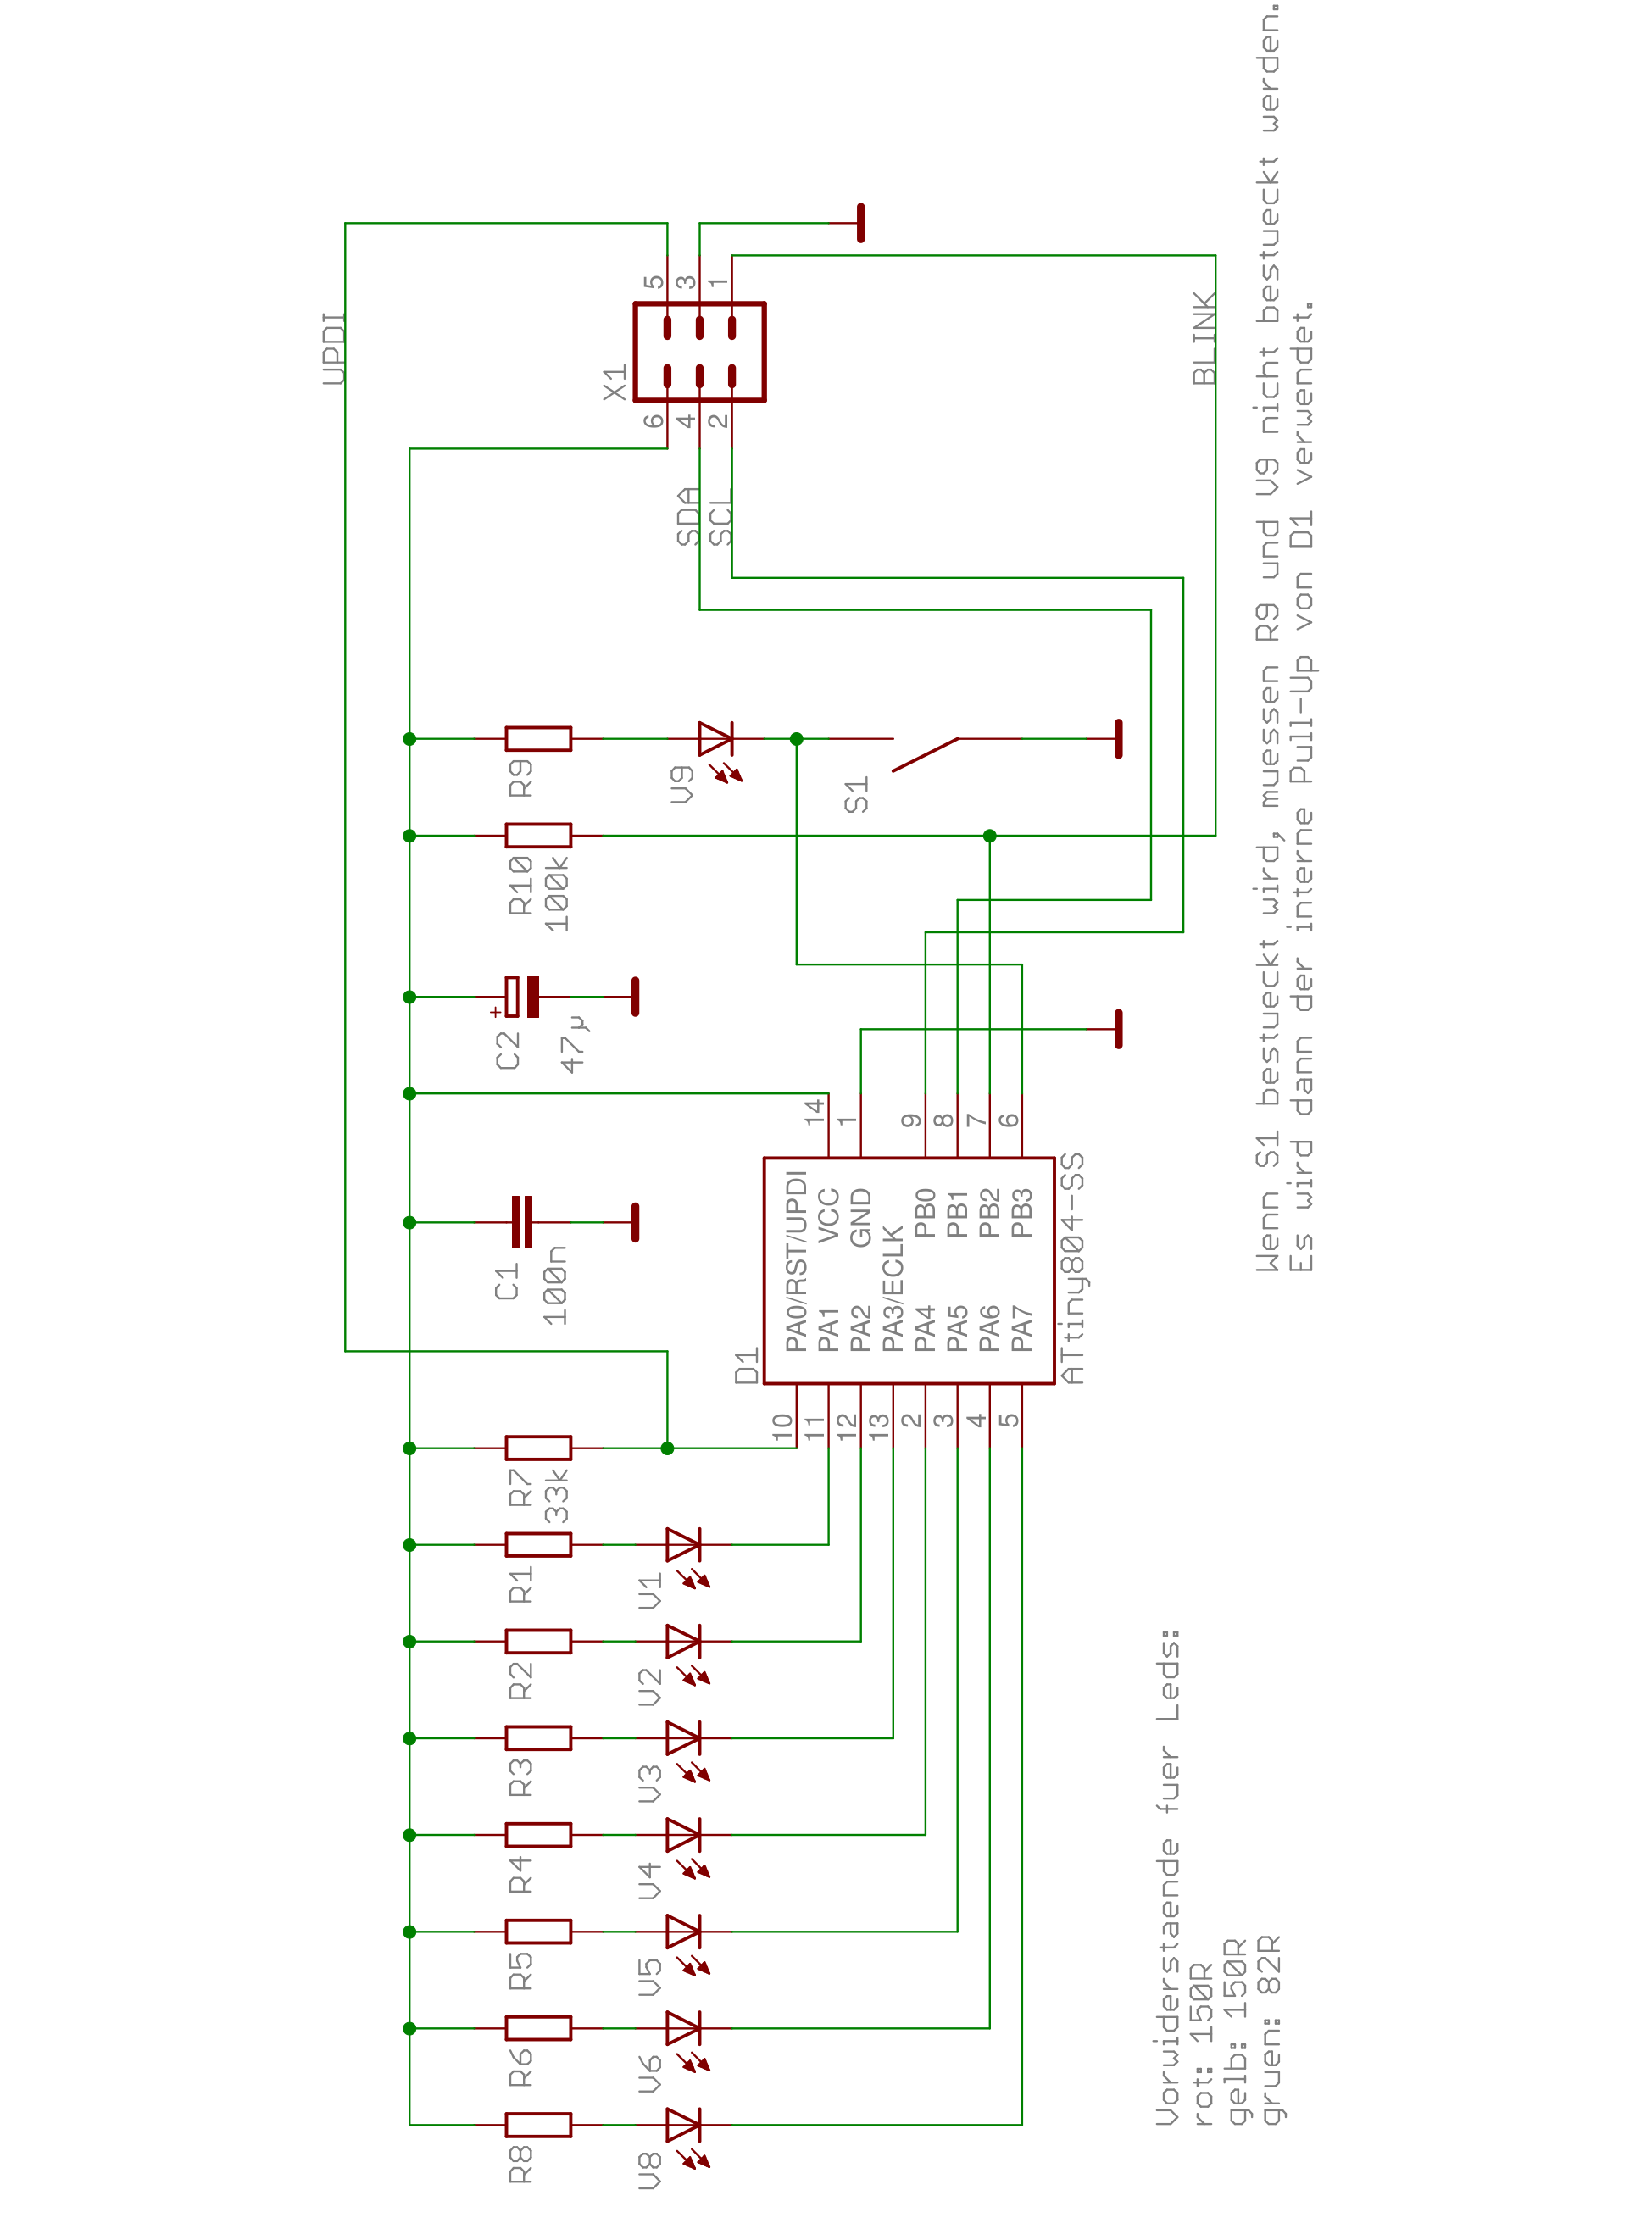
\includegraphics[scale=0.176]{feld_hw.png}
\caption{Schaltplan}
\end{figure}
\begin{figure}[hbtp!]
\centering
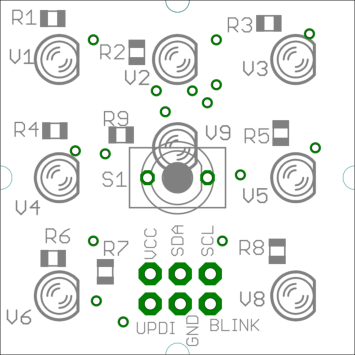
\includegraphics[width=6cm]{feld_hw_top_comp.pdf}
\caption[Bestückungsplan TOP]{Bestückungsplan TOP (Masstab 2:1)}
\end{figure}
\begin{figure}[hbtp!]
\centering
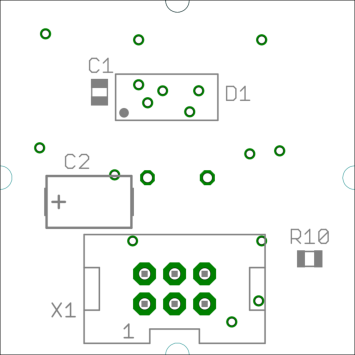
\includegraphics[width=6cm]{feld_hw_bot_comp.pdf}
\caption[Bestückungsplan BOT]{Bestückungsplan BOT (Masstab 2:1)}
\end{figure}
\newpage
\section{Symboltypen}


\subsection{Gleis Gerade (G1)}
\begin{figure}[H]
\centering

\includegraphics[width=3cm]{../folien/g1.png}
\caption{Symbol G1}
\end{figure}
\begin{table}[h!]
\centering
\begin{tabular}{c|c}
\textbf{Pos} & \textbf{Funktion} \\ \hline
4 & LED gelb \\
5 & LED gelb \\
9 & LED gelb
\end{tabular}
\caption{Bestückung G1}
\end{table}


\subsection{Gleis Diagonale (D1)}
\begin{figure}[hbtp]
\centering

\includegraphics[width=3cm]{../folien/d1.png}
\caption{Symbol D1}
\end{figure}
\begin{table}[h!]
\centering
\begin{tabular}{c|c}
\textbf{Pos} & \textbf{Funktion} \\ \hline
3 & LED gelb \\
6 & LED gelb \\
9 & LED gelb
\end{tabular}
\caption{Bestückung D1}
\end{table}


\subsection{Gleis Bogen rechts (B1)}
\begin{figure}[H]
\centering

\includegraphics[width=3cm]{../folien/b1.png}
\caption{Symbol B1}
\end{figure}
\begin{table}[h!]
\centering
\begin{tabular}{c|c}
\textbf{Pos} & \textbf{Funktion} \\ \hline
1 & LED gelb \\
5 & LED gelb \\
9 & LED gelb
\end{tabular}
\caption{Bestückung B1}
\end{table}


\subsection{Gleis Bogen links (B2)}
\begin{figure}[H]
\centering

\includegraphics[width=3cm]{../folien/b2.png}
\caption{Symbol B2}
\end{figure}
\begin{table}[h!]
\centering
\begin{tabular}{c|c}
\textbf{Pos} & \textbf{Funktion} \\ \hline
3 & LED gelb \\
4 & LED gelb \\
9 & LED gelb
\end{tabular}
\caption{Bestückung B2}
\end{table}
\newpage
\subsection{Gleis Funktion gerade (F1)}
Entspricht einer allgemeinen Funktionstaste. Mögliche Funktionen sind z.B. Entkuppler oder Fahrstraßenanfangs oder -endtaste.
\begin{figure}[hbtp]
\centering
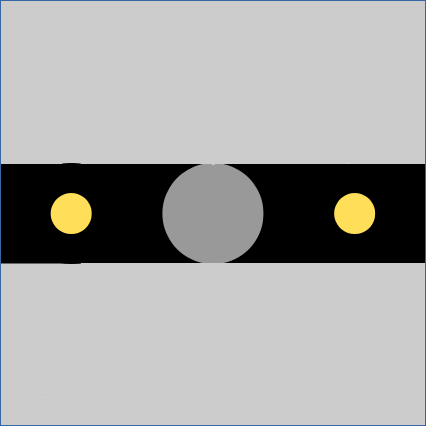
\includegraphics[width=3cm]{../folien/f1.png}
\caption{Symbol F1}
\end{figure}
\begin{table}[h!]
\centering
\begin{tabular}{c|c}
\textbf{Pos} & \textbf{Funktion} \\ \hline
4 & LED gelb \\
5 & LED gelb \\
9 & Taster
\end{tabular}
\caption{Bestückung F1}
\end{table}

\subsection{Gleis Funktion diagonale (F2)}
Entspricht einer allgemeinen Funktionstaste. Mögliche Funktionen sind z.B. Entkuppler oder Fahrstraßenanfangs oder -endtaste.
\begin{figure}[hbtp]
\centering
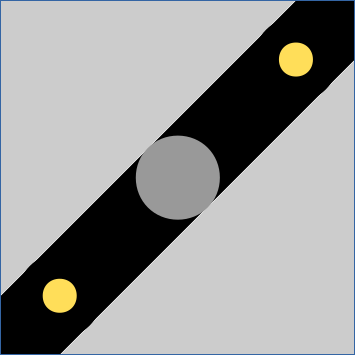
\includegraphics[width=3cm]{../folien/f2.png}
\caption{Symbol F2}
\end{figure}
\begin{table}[h!]
\centering
\begin{tabular}{c|c}
\textbf{Pos} & \textbf{Funktion} \\ \hline
3 & LED gelb \\
6 & LED gelb \\
9 & Taster
\end{tabular}
\caption{Bestückung F2}
\end{table}

\newpage
\subsection{Gleis Funktion Boggen rechts (F3)}
Entspricht einer allgemeinen Funktionstaste. Mögliche Funktionen sind z.B. Entkuppler oder Fahrstraßenanfangs oder -endtaste.
\begin{figure}[hbtp]
\centering
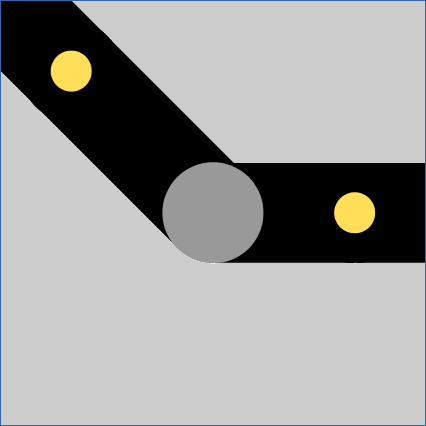
\includegraphics[width=3cm]{../folien/f3.png}
\caption{Symbol F3}
\end{figure}
\begin{table}[h!]
\centering
\begin{tabular}{c|c}
\textbf{Pos} & \textbf{Funktion} \\ \hline
1 & LED gelb \\
5 & LED gelb \\
9 & Taster
\end{tabular}
\caption{Bestückung F3}
\end{table}
 
\subsection{Gleis Funktion Bogen links (F4)}
Entspricht einer allgemeinen Funktionstaste. Mögliche Funktionen sind z.B. Entkuppler oder Fahrstraßenanfangs oder -endtaste.
\begin{figure}[hbtp]
\centering
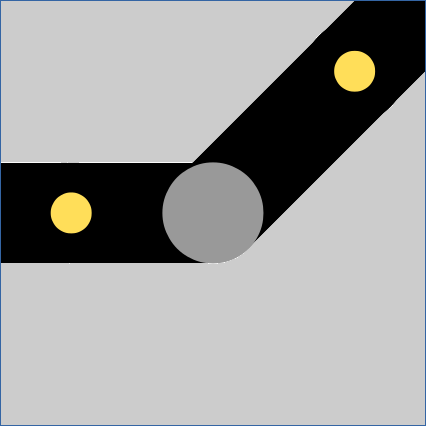
\includegraphics[width=3cm]{../folien/f4.png}
\caption{Symbol F4}
\end{figure}
\begin{table}[h!]
\centering
\begin{tabular}{c|c}
\textbf{Pos} & \textbf{Funktion} \\ \hline
3 & LED gelb \\
4 & LED gelb \\
9 & Taster
\end{tabular}
\caption{Bestückung F4}
\end{table}

\newpage
\subsection{Gleis Weiche rechts (W1)}
Einfache Weiche rechts.
\begin{figure}[hbtp]
\centering

\includegraphics[width=3cm]{../folien/w1.png}
\caption{Symbol W1}
\end{figure}
\begin{table}[h!]
\centering
\begin{tabular}{c|c}
\textbf{Pos} & \textbf{Funktion} \\ \hline
1 & LED gelb \\
4 & LED gelb \\
5 & LED gelb \\
9 & Taster
\end{tabular}
\caption{Bestückung W1}
\end{table}

\subsection{Gleis Weiche links (W2)}
Einfache Weiche links.
\begin{figure}[hbtp]
\centering

\includegraphics[width=3cm]{../folien/w2.png}
\caption{Symbol W2}
\end{figure}
\begin{table}[h!]
\centering
\begin{tabular}{c|c}
\textbf{Pos} & \textbf{Funktion} \\ \hline
4 & LED gelb \\
5 & LED gelb \\
6 & LED gelb \\
9 & Taster
\end{tabular}
\caption{Bestückung W2}
\end{table}

\newpage
\subsection{Gleis Weiche rechts diagonal (W3)}
Einfache Weiche rechts.
\begin{figure}[hbtp]
\centering
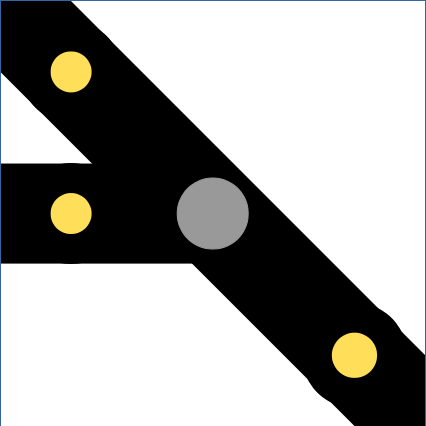
\includegraphics[width=3cm]{../folien/w3.png}
\caption{Symbol W3}
\end{figure}
\begin{table}[h!]
\centering
\begin{tabular}{c|c}
\textbf{Pos} & \textbf{Funktion} \\ \hline
3 & LED gelb \\
5 & LED gelb \\
6 & LED gelb \\
9 & Taster
\end{tabular}
\caption{Bestückung W3}
\end{table}

\subsection{Gleis Weiche links diagonal (W4)}
Einfache Weiche links.
\begin{figure}[hbtp]
\centering
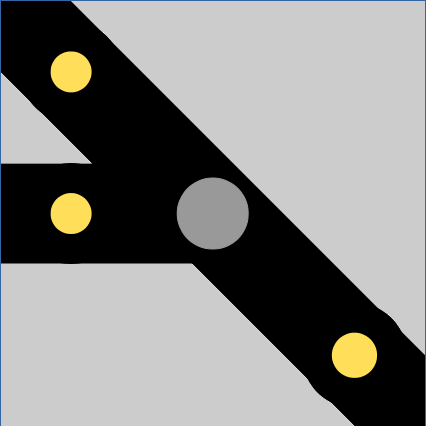
\includegraphics[width=3cm]{../folien/w4.png}
\caption{Symbol W4}
\end{figure}
\begin{table}[h!]
\centering
\begin{tabular}{c|c}
\textbf{Pos} & \textbf{Funktion} \\ \hline
1 & LED gelb \\
4 & LED gelb \\
8 & LED gelb \\
9 & Taster
\end{tabular}
\caption{Bestückung W4}
\end{table}

\newpage
\subsection{Gleis Kreuzungsweiche rechts diagonal (K1)}
Doppelte Kreuzungsweiche.
\begin{figure}[hbtp]
\centering

\includegraphics[width=3cm]{../folien/k1.png}
\caption{Symbol K1}
\end{figure}
\begin{table}[h!]
\centering
\begin{tabular}{c|c}
\textbf{Pos} & \textbf{Funktion} \\ \hline
3 & LED gelb \\
4 & LED gelb \\
5 & LED gelb \\
6 & LED gelb \\
9 & Taster
\end{tabular}
\caption{Bestückung K1}
\end{table}

\subsection{Gleis Kreuzungsweiche links diagonal (K2)}
Doppelte Kreuzungsweiche.
\begin{figure}[hbtp]
\centering
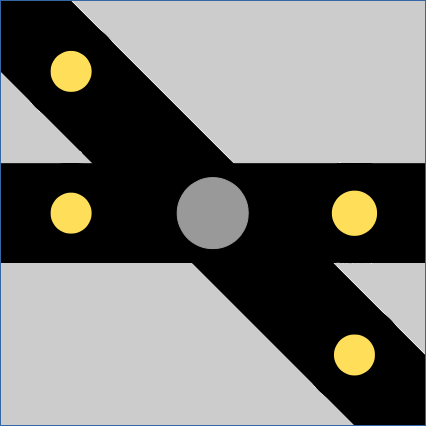
\includegraphics[width=3cm]{../folien/k2.png}
\caption{Symbol K2}
\end{figure}
\begin{table}[h!]
\centering
\begin{tabular}{c|c}
\textbf{Pos} & \textbf{Funktion} \\ \hline
1 & LED gelb \\
4 & LED gelb \\
5 & LED gelb \\
8 & LED gelb \\
9 & Taster
\end{tabular}
\caption{Bestückung K2}
\end{table}


\subsection{Gleis Drewegweiche (3W1)}
Doppelte Kreuzungsweiche.
\begin{figure}[hbtp]
\centering

\includegraphics[width=3cm]{../folien/3w1.png}
\caption{Symbol 3W1}
\end{figure}
\begin{table}[h!]
\centering
\begin{tabular}{c|c}
\textbf{Pos} & \textbf{Funktion} \\ \hline
3 & LED gelb \\
4 & LED gelb \\
5 & LED gelb \\
8 & LED gelb \\
9 & Taster
\end{tabular}
\caption{Bestückung 3W1}
\end{table}


\subsection{Gleis Drewegweiche diagonal (3W2)}
Doppelte Kreuzungsweiche.
\begin{figure}[hbtp]
\centering

\includegraphics[width=3cm]{../folien/3w2.png}
\caption{Symbol 3W2}
\end{figure}
\begin{table}[h!]
\centering
\begin{tabular}{c|c}
\textbf{Pos} & \textbf{Funktion} \\ \hline
1 & LED gelb \\
3 & LED gelb \\
4 & LED gelb \\
6 & LED gelb \\
9 & Taster
\end{tabular}
\caption{Bestückung 3W2}
\end{table}


\subsection{Gleis Drewegweiche diagonal (3W3)}
Doppelte Kreuzungsweiche.
\begin{figure}[hbtp]
\centering

\includegraphics[width=3cm]{../folien/3w3.png}
\caption{Symbol 3W3}
\end{figure}
\begin{table}[h!]
\centering
\begin{tabular}{c|c}
\textbf{Pos} & \textbf{Funktion} \\ \hline
1 & LED gelb \\
4 & LED gelb \\
6 & LED gelb \\
8 & LED gelb \\
9 & Taster
\end{tabular}
\caption{Bestückung 3W3}
\end{table}

\subsection{Gleis Signal Ost (S1)}
Signal Fahrtrichtung Ost.
\begin{figure}[hbtp]
\centering

\includegraphics[width=3cm]{../folien/s1.png}
\caption{Symbol S1}
\end{figure}
\begin{table}[h!]
\centering
\begin{tabular}{c|c}
\textbf{Pos} & \textbf{Funktion} \\ \hline
2 & LED grün \\
3 & LED rot \\
4 & LED gelb \\
5 & LED gelb \\
9 & Taster
\end{tabular}
\caption{Bestückung S1}
\end{table}


\subsection{Gleis Signal West (S2)}
Signal Fahrtrichtung West.
\begin{figure}[hbtp]
\centering

\includegraphics[width=3cm]{../folien/s2.png}
\caption{Symbol S2}
\end{figure}
\begin{table}[h!]
\centering
\begin{tabular}{c|c}
\textbf{Pos} & \textbf{Funktion} \\ \hline
2 & LED grün \\
3 & LED rot \\
4 & LED gelb \\
5 & LED gelb \\
9 & Taster
\end{tabular}
\caption{Bestückung S2}
\end{table}
\newpage
\section{Kommandos}
\subsection{Allgemeines}
Jedes Modul bekommt bei der ersten Programmierung eine Adresse zugewiesen. Aktive Module\footnote{solche mit Taster} bekommen niedrigere als rein passive Module. Dadurch ist sichergestellt, dass Tastenereignisse zeitnah zum Stellwerkscontroller übertragen werden. Die 10bit Adresse ist in der User Row abgelegt.

Als Byte-Reihenfolge wird, soweit nicht explizit anders erwähnt immer Little-Endian verwendet.

\begin{table}[H]
\centering
\begin{tabular}{c|c|l}
\textbf{Bytes} & \textbf{Größe} & \textbf{Beschreibung} \\ \hline
0:1 & 2 & Bits 0:9 10 bit I\textsuperscript{2}C Adresse \\
2 & 1 & Symboltyp 
\end{tabular}
\caption{Aufbau UserRow}
\end{table}

Der allgemeine Kommandoaufbau ist wie folgt\footnote{Da der verwendete Microcontroller nur das erste Adressbyte selbst Prüfen und verarbeiten kann muss das zweite Adressbyte von der Software verwaltet werden.}:

\begin{table}[H]
\centering
\begin{tabular}{c|c|l}
\textbf{Offset} & \textbf{Größe} & \textbf{Beschreibung} \\ \hline
0 & 1 & Adressbits 0:7\\
1 & 1 & Anzahl der Bytes  ohne Prüfsumme (n, max. 8)\\
2 & 1 & CRC8 (siehe \ref{CRC8}) über die nachfolgenden Daten\\
3 & n & Daten
\end{tabular}
\caption{Kommandoaufbau}
\end{table}
Nicht verarbeitbare oder unbekannte Kommandos dürfen nicht quittiert werden, sind aber sonst zu ignorieren. Dies gilt vor allem für Kommandos mit mehr als 8 Datenbytes. So ist sichergestellt, dass in Zukunft auch Kommandos mit mehr Daten implementiert werden können.

Die Anschließende Kommandobeschreibung zeigt nur die Datenbytes !

\subsubsection{Lange Adressen}
Bei kurzen Adressen wird die Adressfilterung von der Hardware durchgeführt. Byte 0 ist dann undefiniert. 

Bei langen Adressen, werden nur die oberen zwei Adressbits von der Hardware gefiltert. Byte 0 enthält dann die Adressbits 0-7.

\subsection{Housekeeping}
\label{sec:Housekeeping}
In dieser Kommandogruppe liegen alle Kommandos die der Aktivierung und Konfigurierung der Module liegen. 
\begin{figure}[H]
\centering
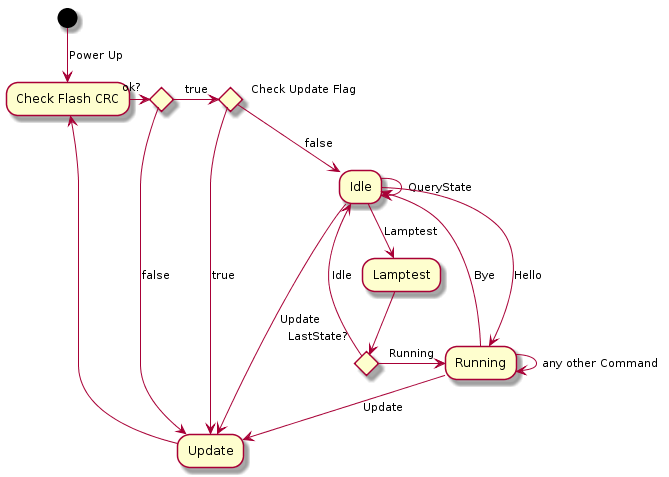
\includegraphics[scale=0.5]{global_activity.png}
\caption{Globales Zustandsdiagramm}
\end{figure}

\subsubsection{QueryState}
\label{sec:QueryState}
Dieses Kommando dient zum Abfragen des aktuellen Zustands des Moduls.
\begin{table}[H]
\centering
\begin{tabular}{c|c|l|l}
\textbf{Offset} & \textbf{Länge} & \textbf{Wert} & \textbf{Beschreibung} \\ \hline
0 & 1 & 0x01 & Kommando QueryState 
\end{tabular}
\caption{QueryState Request}
\end{table}

\begin{table}[H]
\label{QUERYSTATE_RESP}
\centering
\begin{tabular}{c|c|c|l}
\textbf{Offset} & \textbf{Länge} & \textbf{Wert} & \textbf{Beschreibung} \\ \hline
0 & 1 & s & Aktueller State\\
1 & 1 & l & Aktueller Status der LEDs\\
2 & 1 & b & Blinkmaske (Positionen mit 1 blinken)\\
3 & 1 & t & div. Flags\\
4 & 1 & va & Version major\\
5 & 1 & vi & Version minor\\
6 & 2 & bu & Build number
\end{tabular}
\caption{QueryState Response}
\end{table}

\begin{table}[H]
\centering
\begin{tabular}{c|c}
\label{POSMASK}
\textbf{Bit} & \textbf{LED Position} \\ \hline
0 & 1 \\
1 & 2 \\
2 & 3 \\
3 & 4 \\
4 & 5 \\
5 & 6 \\
6 & 8 \\
7 & 9
\end{tabular}
\caption{LED Positionen}
\end{table}


\subsubsection{Hello}
\label{sec:Hello}
Dieses Kommando aktiviert das Modul. Ohne Aktivierung muss sich ein Modul passiv verhalten (vor allem darf es nicht mehr Strom als notwendig.
\begin{table}[H]
\centering
\begin{tabular}{c|c|l|l}
\textbf{Offset} & \textbf{Länge} & \textbf{Wert} & \textbf{Beschreibung} \\ \hline
0 & 1 & 0x02 & Kommando Hello 
\end{tabular}
\caption{Hello Request}
\end{table}
Antwort wie unter \ref{QUERYSTATE_RESP} QueryState.

\subsubsection{Lamptest}
\label{sec:Lamptest}
Führt einen Lamptest durch. Die selektierten Tests werden solange in einer Endlosschleife durchgeführt bis das Kommando mit dem Flagbyte=0 übertragen wird. Jeder Test wird eine Sekunde lang angezeigt.
\begin{table}[H]
\centering
\begin{tabular}{c|c|c|l}
\textbf{Offset} & \textbf{Länge} & \textbf{Wert} & \textbf{Beschreibung} \\ \hline
0 & 1 & 0x03 & Kommando Lamptest\\
1 & 1 & f & Durchzuführende Tests (siehe Tabelle unten). 
\end{tabular}
\caption{Lamptest Request}
\end{table}

\begin{table}[H]
\label{LAMPTEST_FLAGS}
\centering
\begin{tabular}{c|l}
\textbf{Bit} & \textbf{Test} \\ \hline
0 & Alle LEDs an bei 100\% Helligkeit\\
1 & Jede LED einzeln bei 100\% Helligkeit\\
2 & Alle LEDs bei 20\% Helligkeit\\
3 & Alle LEDs bei 40\% Helligkeit\\
4 & Alle LEDs bei 60\% Helligkeit\\
5 & Alle LEDs bei 80\% Helligkeit\\
6 & Alle LEDs aus
\end{tabular}
\caption{Lamptest Flags}
\end{table}

\subsubsection{Update}
\label{sec:Update}
Wechsel in den Modus Update.
\begin{table}[H]
\centering
\begin{tabular}{c|c|c|l}
\textbf{Offset} & \textbf{Länge} & \textbf{Wert} & \textbf{Beschreibung} \\ \hline
0 & 1 & 0x04 & Kommando Update
\end{tabular}
\caption{Lamptest Request}
\end{table}

\subsubsection{Bye}
\label{sec:Bye}
Wechsel in den Modus Idle.
\begin{table}[H]
\centering
\begin{tabular}{c|c|c|l}
\textbf{Offset} & \textbf{Länge} & \textbf{Wert} & \textbf{Beschreibung} \\ \hline
0 & 1 & 0x05 & Kommando Bye
\end{tabular}
\caption{Bye Request}
\end{table}

\subsubsection{Healtcheck}
\label{sec:Healthcheck}
Führt eine Messung der Versorgungsspannung, bei Leerlauf (min. möglicher Stromverbrauch des Elements), und eine Messung bei Vollast (max. möglicher Stromverbrauch). Dieses Kommando steht im Modus Update nicht zur Verfügung.

Die Vollastmessungen müssen am Ende der Vollastperiode durchgeführt werden.
\begin{table}[H]
\centering
\begin{tabular}{c|c|c|l}
\textbf{Offset} & \textbf{Länge} & \textbf{Wert} & \textbf{Beschreibung} \\ \hline
0 & 1 & 0x0c & Kommando Healtchcheck \\
1 & 1 & t & Dauer der Vollastperiode in Sekunden.
\end{tabular}
\caption{Healthcheck Request}
\end{table}
\begin{table}[H]
\centering
\begin{tabular}{c|c|c|l}
\textbf{Offset} & \textbf{Länge} & \textbf{Wert} & \textbf{Beschreibung} \\ \hline
0 & 1 & ul & Spannung bei Leerlauf in 0,1 V\\
1 & 1 & ul & Spannung bei Vollast in 0,1 V\\
4 & 2 & t & Chiptemeratur bei Vollast in Kelvin
\end{tabular}
\caption{Healthcheck Response}
\end{table}


\subsection{Update}
Jedes Modul wird initial mit einem Bootloader programmiert.

Es gibt zwei Wege wie der Bootloader aktiviert wird:
\begin{itemize}
 \item CRC Fehler des Programms (siehe \ref{CHECK_CRC} und \ref{CRC16}).
 \item Wechsel in den Modus Update. 
\end{itemize}
  
\subsubsection{PageLoad}
\label{sec:PageLoad}
Übertragen der Daten eine Seite (64 Byte). Dieses Kommando ist ein Kommando mit überlangen Datenblock. Es muss immer eine vollständige Seite übertragen werden. Nicht definierte Bytes müssen mit 0xff übertragen werden.
\begin{table}[H]
\centering
\begin{tabular}{c|c|c|l}
\textbf{Offset} & \textbf{Länge} & \textbf{Wert} & \textbf{Beschreibung} \\ \hline
0 & 1 & 0x06 & Kommando Page Load\\
1 & 64 & d & Daten
\end{tabular}
\caption{Page Load Request}
\end{table}

\subsubsection{PageProgram}
\label{sec:PageProgram}
Übertragen der zuletzt gesendeten Speicherseite ins Flash. Sollte die zu Programmierende Seite in den Bootsektor zeigen, ist das Programm zu ignorieren. Der Programmiermodus wird durch das Kommand PageProgram mit Offset 0 (ist immer im Bootsektor) beendet.
\begin{table}[H]
\centering
\begin{tabular}{c|c|c|l}
\textbf{Offset} & \textbf{Länge} & \textbf{Wert} & \textbf{Beschreibung} \\ \hline
0 & 1 & 0x07 & Kommando PageProgram\\
1 & 2 & o & Page Address
\end{tabular}
\caption{PageProgram Request}
\end{table}

\subsubsection{CheckCRC}
\label{CHECK_CRC}
\label{sec:CheckCRC}
Überprüfen des Flash Speichers.
\begin{table}[H]
\centering
\begin{tabular}{c|c|c|l}
\textbf{Offset} & \textbf{Länge} & \textbf{Wert} & \textbf{Beschreibung} \\ \hline
0 & 1 & 0x08 & Kommando CheckCRC\\
\end{tabular}
\caption{CheckCRC Request}
\end{table}
\begin{table}[H]
\centering
\begin{tabular}{c|c|c|l}
\textbf{Offset} & \textbf{Länge} & \textbf{Wert} & \textbf{Beschreibung} \\ \hline
0 & 1 & b & Result\\
\end{tabular}
\caption{CheckCRC Respone}
\end{table}
\begin{table}[H]
\centering
\begin{tabular}{c|l}
\textbf{Bit} & \textbf{Bereich} \\ \hline
0 & Boot OK\\
1 & Application OK\\
\end{tabular}
\caption{CheckCRC Result}
\end{table}


\subsection{Running}
Diese Betriebsart stellt den eigentliche Betrieb des Moduls dar.
\subsubsection{Lamp}
\label{sec:Lamp}
Schalten der LEDs.
\begin{table}[H]
\centering
\begin{tabular}{c|c|c|l}
\textbf{Offset} & \textbf{Länge} & \textbf{Wert} & \textbf{Beschreibung} \\ \hline
0 & 1 & 0x09 & Kommando Lamp\\
1 & 1 & b & Status der einzelnen Leds (siehe Tabelle \ref{POSMASK})\\
2 & 1 & m & Blinkmaske (siehe Tabelle \ref{POSMASK})
\end{tabular}
\caption{Lamp Request}
\end{table}

\subsubsection{KeyQuery}
\label{sec:KeyQuery}
Abfragen des Tastenstatus.
\begin{table}[H]
\centering
\begin{tabular}{c|c|c|l}
\textbf{Offset} & \textbf{Länge} & \textbf{Wert} & \textbf{Beschreibung} \\ \hline
0 & 1 & 0x0a & Kommando KeyQuery\\
1 & 1 & b & Wenn die Taste gedrückt ist 1 sonst 0
\end{tabular}
\caption{KeyQuery Request}
\end{table}
\begin{table}[H]
\label{tab:keyquery_response}
\centering
\begin{tabular}{c|c|c|l}
\textbf{Offset} & \textbf{Länge} & \textbf{Wert} & \textbf{Beschreibung} \\ \hline
1 & 1 & b & Wenn die Taste gedrückt ist 1 sonst 0
\end{tabular}
\caption{KeyQuery Response}
\end{table}

\subsubsection{KeyEvent}
\label{sec:KeyEvent}
Dieses Kommando wird vom Modul ausgelöst.
\begin{table}[H]
\centering
\begin{tabular}{c|c|c|l}
\textbf{Offset} & \textbf{Länge} & \textbf{Wert} & \textbf{Beschreibung} \\ \hline
0 & 1 & 0x0b & Kommando KeyEvent\\
1 & 2 & a & Adresse des Moduls\\
3 & 1 & b & Wenn die Taste gedrückt ist 1 sonst 0
\end{tabular}
\caption{KeyEvent Request}
\end{table}



\newpage
\appendix
\section{Berechnung CRC-8}
\label{CRC8}
\begin{alltt}
const datalen;
var crc: Byte;
var data: Array of Byte[datalen];
var n: Integer;
begin
  crc:= 0;
  for n:=0 to datalen-1
    crc := updcrc8(data[n],crc); 
  end
  return crc;
end
\end{alltt}
mit
\begin{alltt}
updcrc8(\(\downarrow\) b,\(\downarrow\) crc): Byte
  b, crc : Byte;
var
  n : Byte;
  s : Byte;
begin
  for n:=1 to 8
    s := b & 0x01;
    if (crc and 0x80)<> 0 then
      crc := (crc * 2 + s) ^ 0x07;
    else
      crc := (crc * 2 + s);
    end
    b := b >> 1;
  end
  return crc;
end
\end{alltt}

\section{Berechnung CRC-16}
\label{CRC16}
\begin{alltt}
const datalen;
var crc: Word;
var data: Array of Byte[datalen];
var n: Integer;
begin
  crc:= 0;
  for n:=0 to datalen-1
    crc := updcrc16(data[n],crc); 
  end
  return crc;
end
\end{alltt}
mit
\begin{alltt}
updcrc16(\(\downarrow\) b,\(\downarrow\) crc): Word
  b : Byte;
  crc: Word;
var
  n : Byte;
  s : Byte;
begin
  for n:=1 to 8
    s := b & 0x01;
    if (crc and 0x8000)<> 0 then
      crc := (crc * 2 + s) ^ 0x1021;
    else
      crc := (crc * 2 + s);
    end
    b := b >> 1;
  end
  return crc;
end
\end{alltt}

\section{Kommandocodes}
\begin{table}[H]
\centering
\begin{tabular}{c|l|l}
\textbf{Code} & \textbf{Name} & \textbf{Abschnitt} \\ \hline
0x01 & QueryState & \ref{sec:QueryState}\\
0x02 & Hello & \ref{sec:Hello}\\
0x03 & Lamptest & \ref{sec:Lamptest}\\
0x04 & Update & \ref{sec:Update}\\
0x05 & Bye & \ref{sec:Bye}\\
0x06 & PageLoad & \ref{sec:PageLoad}\\
0x07 & PageProgram & \ref{sec:PageProgram}\\
0x08 & CheckCRC & \ref{sec:CheckCRC}\\
0x09 & Lamp & \ref{sec:Lamp}\\
0x0a & KeyQuery & \ref{sec:KeyQuery}\\
0x0b & KeyEvent & \ref{sec:KeyEvent}\\
0x0c & Healthcheck & \ref{sec:Healthcheck}
\end{tabular}
\caption{Kommandocodes}
\end{table}



\nocite{*}

\addcontentsline{toc}{section}{Literatur und Quellen}
\printbibliography
\end{document}